%%%%%%%%%%%%%%%%%%%%%%%%%%%%%%%%%%%%%%%%%
% Universitat de Girona Laboratory Report
% LaTeX Template
%
% This template has been downloaded from:
% http://www.LaTeXTemplates.com
%
% Original author:
% Linux and Unix Users Group at Virginia Tech Wiki 
% (https://vtluug.org/wiki/Example_LaTeX_chem_lab_report)
%
% License:
% CC BY-NC-SA 3.0 (http://creativecommons.org/licenses/by-nc-sa/3.0/)
%
%%%%%%%%%%%%%%%%%%%%%%%%%%%%%%%%%%%%%%%%%

%----------------------------------------------------------------------------------------
%	PACKAGES AND DOCUMENT CONFIGURATIONS
%----------------------------------------------------------------------------------------

\documentclass{article}

\usepackage{graphicx} % Required for the inclusion of images
\usepackage{natbib} % Required to change bibliography style to APA
\usepackage{amsmath} % Required for some math elements 
\usepackage{geometry}
\usepackage{color}
 \geometry{
 a4paper,
 left=30mm,
 right=30mm,
 top=30mm,
 bottom=25mm,
 }
 
\setlength\parindent{0pt} % Removes all indentation from paragraphs
\setcounter{MaxMatrixCols}{50}


%\usepackage{times} % Uncomment to use the Times New Roman font

%----------------------------------------------------------------------------------------
%	DOCUMENT INFORMATION
%----------------------------------------------------------------------------------------

\title{The Rotational Plane Sweep \\ Autonomous Robots \\ LAB 02} % Title

\author{Taner \textsc{GUNGOR}} % Author name

\date{\today} % Date for the report

\begin{document}

\maketitle % Insert the title, author and date

\begin{center}
\begin{tabular}{l r}
Deadline: & April 12, 2015 \\ % Deadline date of the experiment
%Partners: & James Smith \\ & Mary Smith \\ % Partner names
Instructor: & Marc Carreras % Instructor/supervisor
\end{tabular}
\end{center}

% If you wish to include an abstract, uncomment the lines below
% \begin{abstract}
% Abstract text
% \end{abstract}


%----------------------------------------------------------------------------------------
%	SECTION 1
%----------------------------------------------------------------------------------------

\section{Objective}

The aim of this lab is to understand the rotational plane sweep algorithm to build a visibility graph and implement it in Matlab.

\section{Introduction}

The rotational plane sweep is a path planning algorithm based on topological maps. It is one of the most powerful method of intelligent robot navigation. The basic concepts and details of the algorithm are going to be explained in the next chapter. After that, we are going to see the results.


%----------------------------------------------------------------------------------------
%	SECTION 2
%----------------------------------------------------------------------------------------

\section{The Algorithm}

Topological map is a simplified map with only relationship between points. It can be represented as a graph:

\begin{itemize}
  \item nodes are real positions
  \item edges join positions in the free space.
\end{itemize}

They include the distance. It is easy to find a path in a topological map. So, the only problem is how to build a topological map? We are going to create visibility graph.
\\

In order to create visibility graph. We should define for a 2D polygonal configuration space

\begin{itemize}
  \item The nodes $v_{i}$ of the visibility graph include the start location, the goal location, and all the vertices of the configuration space obstacles.
  \item The graph edges $e_{ij}$ are straight-line segments that connect two line-of-sight nodes $v_{i}$ and $v_{j}$, i.e., 
\end{itemize}

\begin{equation}
e_{ij} \neq \emptyset \Longleftrightarrow sv_{i} + (1 - s)v_{j} \in cl(Q_{free}) \forall s \in [0, 1]
\end{equation}

Construction of the visibility graph with n nodes has complexity $n^{3}$ for all nodes; for all potential edges; for all obstacle edges wich can be reduced with the Rotational Plane Sweep Algorithm.
\\

If we use visibility graph construction with brute force, it takes a lot of computions and time. However, if we use the rotational plane sweep algorithm for building the visibility graph, the total time complexity of $n^{2} logn$ and you should do the followings:

\begin{itemize}
  \item A rotating half-line emanating from any vertex will be used to determine the vertices which are visible.
  \item The half-line has to stop only in the directions in which there is a vertex.
  \item At each vertex angle, a list of edges which intersect the beam will be updated (list S).
  \item Since the line rotates following the sorted list of vertex angles, list $\varepsilon$, the updating of the S list consists only on adding or removing the edges that contain the candidate vertex.
  \item Then, to determine if the vertex is visible, only intersection with lines contained in the S list, that are closer than the candidate vertex, have to be checked.
\end{itemize}

The algorithm uses a line which start point, let call it reference vertex, and end point is coordinates of all other vertices of the all obstacles, including start and goal positions of the robot, let call them examining vertices. The angle of the sweeping line set to zero initially, and begins to sweep counter-clockwise from 0 to 2$\pi$ [rad]. 
\\

While this sweeping procedure, edges of the obstacles added to or removed from dynamic edge list S according to join which vertex of the obstacles. At each instant vertices list is checked for whether reference and examining vertices have line-of-sight or not.
\\

\subsection{Find the angle list $\varepsilon$}

As explained above, the algorithm uses a line that starts from the first vertex to the other vertices. In this step, we should find the angles of these lines and put them to the angle list $\varepsilon$. After finding angle for all the vertices, we should sort them ascending order. Now, we are ready to check the intersection. But we need to do one more thing before passing the next section. We should initialize the list S. In order to initialize it, we should set the angle of the sweeping line to zero which is green line in the figure 1 and put the intersected line segments to the list S.

\begin{figure}[!h]
\begin{center}
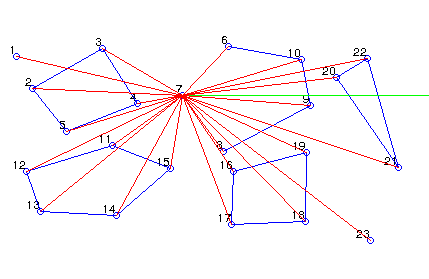
\includegraphics[scale=0.9]{00}
\caption{Find the angle list $\varepsilon$.}
\end{center}
\end{figure}

When you call the following function, it is going to return the angle list $\varepsilon$ which contains the positive angle, the original angle and the index of the other vertex.
\\

\hspace{1cm}\texttt{[ angles ] = calculate\_angle( current\_vertex, vertices );}
\\

\hspace{1cm}\texttt{angles =}

\hspace{2cm}\texttt{0.0000 \ \ 0.0000 \ \ 7 [CURRENT VERTEX = 7]}

\hspace{2cm}\texttt{0.1438 \ \ 0.1438 \ 20}

\hspace{2cm}\texttt{0.2463 \ \ 0.2463 \ 22}

\hspace{2cm}\texttt{\vdots \ \ \ \ \ \ \ \ \vdots \ \ \ \ \ \ \ \ \vdots }

\hspace{2cm}\texttt{5.7504 \ -0.5328 \ 19}

\hspace{2cm}\texttt{5.8801 \ -0.4031 \ 21}

\hspace{2cm}\texttt{6.1843 \ -0.0989 \ \ 9}

\subsection{Check the intersection}

In this section, we should \textbf{choose the line segment that has the smallest distance and not belong to the current vertex} from the list S. Then we should check if there is an intersection between this line segment and the edge which is between current vertex and target vertex. If the intersection exists, we should not add this edge to the visibility graph. If there is not an intersection, we should add it to the visibility graph.
\\

Let's make an example. But before it, I want to explain the structure of the list S which I use in Matlab. It contains the distance and the indices of the vertices creates that line segment like below. Now, we can make our example. As you can see from the figure 2, after initialization we have 3 edges [(10, 9), (21, 20), (22, 21)] in the list S and their distances to the current vertex 7.
\\

\hspace{1cm}\texttt{list\_S =}

\hspace{2cm}\texttt{3.5317 \ \ 10 \ \ \ 9 [SMALLEST DISTANCE = (10, 9)]}

\hspace{2cm}\texttt{5.3844 \ \ 21 \ \ 20}

\hspace{2cm}\texttt{5.8805 \ \ 22 \ \ 21}

\begin{figure}[!h]
\begin{center}
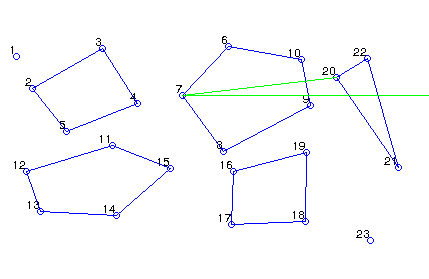
\includegraphics[scale=0.9]{09}
\caption{Check the intersection between (7, 20) and (10, 9) which is the smallest line segment in the list S}
\end{center}
\end{figure}

We should draw a line from the current vertex 7 to the 20th vertex in the graph and we should check if there is an intersection between this line and the other line segment (10, 9) which has the smallest distance in the list S. After checking, we know that there is an intersection, so we do not add this edge to the visibility graph. One by one, we should check for all the vertices. Now, let's draw a line from the current vertex 7 to the 3rd one in the graph and check if there is an intersection between this line and the other line segment (8, 7) which has the smallest distance in the list S. But here, we have special condition. The line segment (8, 7) belongs to the vertex 7, so we cannot take this line segment. We should get the second smallest lines segment in the list S. But, there is not a second smallest line segment in the list S. So, we add this line to the visibility graph.
\\

\hspace{1cm}\texttt{list\_S =}

\hspace{2cm}\texttt{1.1261 \ \ \ 8 \ \ \ 7 [SMALLEST DISTANCE = (10, 9)]}

\begin{figure}[!h]
\begin{center}
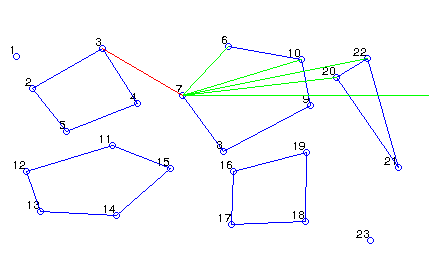
\includegraphics[scale=0.9]{10}
\caption{Check the intersection between (7, 3) and (8, 7) which is the smallest line segment in the list S (But here be careful, (8, 7) belongs to the current vertex. So we do not need to check it. We can easily say there is no any intersection)}
\end{center}
\end{figure}

\begin{figure}[!h]
\begin{center}
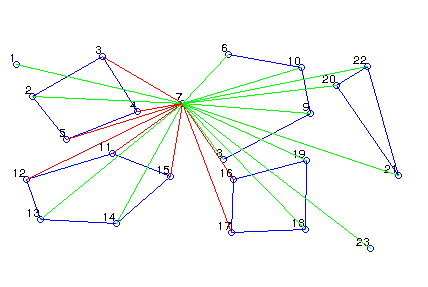
\includegraphics[scale=0.9]{01}
\caption{Red lines are added to the visibility graph, green lines are not added to the visibility graph because of the intersection (Current vertex is 7)}
\end{center}
\end{figure}

\subsection{Update the list S}

After checking whether intersection exists or not, we should update the list S. if $v_{i}$ is the beginning of an edge and this edge not in the list S, then we should add it to the list. And also we should check that if the $v_{i}$ is the end of the edge in the list S, then we should remove it from the list. During adding process, we should also calculate the distance from the current vertex to the current line segment.
\\

Let's make an example to understand better. As you can see from the figure 5, we draw a straight line whose angle is 0 and put all the edges ((3, 2), (4, 3), (7, 6), (10, 6)) that intersect with this line to the list S with their distances 1.8024, 3.0549, 5.3243, 6.8616 respectively. After that we should look at each vertex one by one according to its angle(ascending order) like figures 6 and 7.

\begin{figure}[!h]
\begin{center}
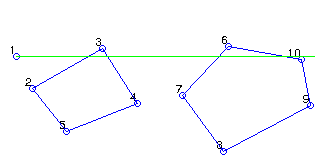
\includegraphics[scale=1.0]{02}
\caption{Initialize the list S [(3, 2), (4, 3), (7, 6), (10, 6)] by adding all intersected edges.}
\end{center}
\end{figure}

\begin{figure}[!h]
\begin{center}
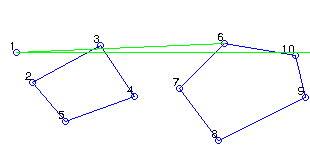
\includegraphics[scale=1.0]{03}
\caption{Check the visibility (Do not add the (1, 6) to the visibility graph), update the list S[(3, 2), (4, 3)] by deleting all the edges that is the end of the edge and add all the edges that is the beginning of the edge.}
\end{center}
\end{figure}

\begin{figure}[!h]
\begin{center}
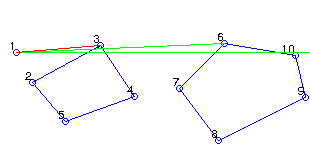
\includegraphics[scale=1.0]{04}
\caption{Check the visibility (Add the (1, 3) to the visibility graph), update the list S[] by deleting all the edges that is the end of the edge and add all the edges that is the beginning of the edge.}
\end{center}
\end{figure}

\subsubsection{Find the distance of each segment line}

We should be careful here to calculate the distance of each line segment. Because In the first time, I calculated the distance from the current vertex to \textbf{the line}. But it creates a problem when we are sorting the edges according to their distances. You can see this problematic method from the figure 8.
\\

So instead of calculating the distance from current vertex to the line, we should compute the distance from current vertex to \textbf{the line segment}. The line segment has 2 points. I calculated the distances from the current vertex to these 2 points and took their average. You can see the idea from the figure 9. 

\begin{figure}[!h]
\begin{center}
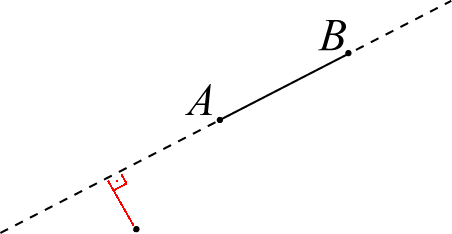
\includegraphics[scale=1.5]{05}
\caption{The distance between line and the vertex (Problematic method).}
\end{center}
\end{figure}

\begin{figure}[!h]
\begin{center}
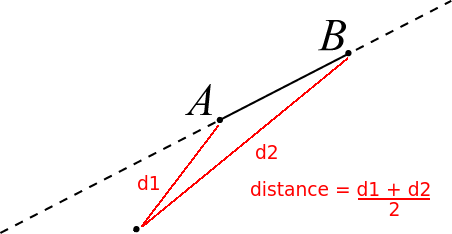
\includegraphics[scale=1.5]{06}
\caption{The distance between line segment and the vertex.}
\end{center}
\end{figure}

By doing this calculation for all the line segments, help us to find the correct line segment that has the smallest distance during the 'checking the intersection' step without facing any problems.




%----------------------------------------------------------------------------------------
%	SECTION 3
%----------------------------------------------------------------------------------------

\section{The results \& conclusion}

From the figures 10 and 11, you can see that the algorithm is working in both graphs. This laboratory work was very helpful to understand the theoretical background of the rotational plane sweep algorithm. It helped me to explore more information about it and how to apply to the robot navigation.

\begin{figure}[!h]
\begin{center}
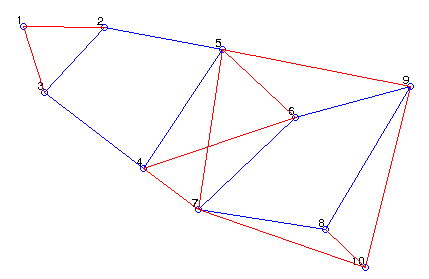
\includegraphics[scale=1.0]{07}
\caption{The result of the rotational plane sweep algorithm. [Small graph]}
\end{center}
\end{figure}

\begin{figure}[!h]
\begin{center}
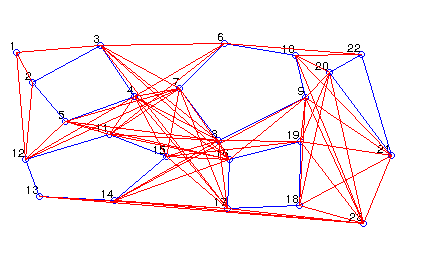
\includegraphics[scale=1.0]{08}
\caption{The result of the rotational plane sweep algorithm. [Big graph]}
\end{center}
\end{figure}


%----------------------------------------------------------------------------------------
%	BIBLIOGRAPHY
%----------------------------------------------------------------------------------------

\bibliographystyle{apalike}

\bibliography{sample}

%----------------------------------------------------------------------------------------

\end{document}